\documentclass[12pt,a4paper,twoside]{book}
\usepackage[utf8]{inputenc}
\usepackage{amsmath}
\usepackage{amsfonts}
\usepackage{amssymb}
\usepackage{graphicx}
\usepackage[inner=3.00cm, outer=2.50cm, top=3.00cm, bottom=3.00cm]{geometry}
\usepackage[slovene]{babel}
\usepackage{babelbib}
\usepackage{titlesec}
\usepackage{fancyhdr}
\usepackage{eurosym}
\usepackage{url}
\author{Luka Horvat}
\title{Dobre prakse pri razvoju računalniških iger}

\graphicspath{{images/}}
%Paragraph indenting, title spacing and line spacing
\setlength{\parindent}{0pt}
\setlength{\parskip}{1em}
\renewcommand{\baselinestretch}{1.5}

% Remove big chapter text
\titleformat{\chapter}{\bfseries\LARGE}{\thechapter}{1em}{\LARGE\textbf}

%Header/footer
\pagestyle{fancy}
\fancyhf{}
\fancyfoot[LE,RO]{\thepage}
\renewcommand{\headrulewidth}{0pt}
\renewcommand{\footrulewidth}{0pt}

%Initial pages are in Roman numbering
\pagenumbering{Roman}
\begin{document}
	
%First page
\thispagestyle{empty} 
\begin{center}
{\large 
UNIVERZA V MARIBORU\\
FAKULTETA ZA ELEKTROTEHNIKO,\\
RAČUNALNIŠTVO IN INFORMATIKO\\
}

\vspace{\fill}
{\LARGE Luka Horvat}\\

\vspace{1cm}
\textsc{\textbf{\LARGE
		DOBRE PRAKSE PRI RAZVOJU RAČUNALNIŠKIH IGER\\}}

\vspace{1cm}
{\LARGE Magistrsko delo}

\vfill
{\Large Maribor, februar 2018}
\newpage
\end{center}

%Empty page
\ \thispagestyle{empty}
\newpage

%Second page
\thispagestyle{empty} 
\begin{center}	
\vspace*{\fill}
\textsc{\textbf{\LARGE
		Dobre prakse pri razvoju računalniških iger\\
	}}
{\large\textbf{Magistrsko delo\\}
	
}
\vspace{\fill}
\begin{tabbing}
\hspace*{4cm}\=\hspace*{3cm}\= \kill
Študent: \> Luka Horvat\\
Študijski program: \> Študijski program 2. stopnje\\
\>Računalništvo in informacijske tehnologije\\
Mentor: \> doc. dr. Matej Črepinšek
\end{tabbing}
\end{center}
\newpage

%Empty page
\ \thispagestyle{empty}
\newpage

%Sklep
\thispagestyle{empty}
Tukaj pride sklep o potrjeni temi.
\newpage

%Empty page
\ \thispagestyle{empty}
\newpage

%Povzetek v slovenskem jeziku
\chapter*{Dobre prakse pri razvoju računalniških iger}
\thispagestyle{fancy}
\setcounter{page}{1}
\textbf{Ključne besede:} beseda1

\textbf{UDK:} 123

\textbf{Povzetek}\newline
\textit{Povzetek do maksimalne dolžine 100 besed}
\cleardoublepage

%Povzetek v angleškem jeziku
\chapter*{Dobre prakse pri razvoju računalniških iger}
\thispagestyle{fancy}
\textbf{Key words:} word 1

\textbf{UDK:} 123

\textbf{Abstract:}\newline
\textit{Povzetek do maksimalne dolžine 100 besed}
\cleardoublepage

%Kazalo
\tableofcontents
\thispagestyle{fancy}

%Kazalo vsebine
\listoffigures
\thispagestyle{fancy}

%Content
%Uvod
\chapter{Uvod}
%Page numbering and style changes here
\setcounter{page}{1}
\pagenumbering{arabic}
\thispagestyle{fancy}

Računalniške igre so ena izmed največjih panog v zabaviščni industriji. Skozi leta pa se njihov delež samo povečuje. Dandanes se je že skoraj vsak posameznik srečal z računalniškimi igrami, ali jih neposredno igra v svojem prostem času, ali pa so se posredno vključile v kulturo okoli posameznika. Računalniške igre in še posebej like iz njih velikokrat vidimo v drugih medijih kot so filmi, serije, reklame ter tiskano gradivo. Kdo pa si danes pod imenom Mario ne predstavlja vodovodarja v rdečem kombinezonu ter velikimi brki?

Računalniške igre privabljajo vedno več podjetij in individualnih razvijalcev, ki poskušajo zavzet svoj prostor v tej industriji. Samo izdelovanje računalniških iger pa uvrstimo pod razvoj programske opreme, ki je izredno kompleksen in zahteva potrebna znanja iz več različnih panog. Napredek tehnologije pa je že skoraj vsakemu posamezniku omogočil preprost vstop v ta proces. Dandanes je na voljo toliko različnih orodij, knjig, procesov in ustaljenih praks, ki so na voljo posamezniku, vendar se v oceanu podatkov hitro izgubijo. Tako smo si kot cilj tega magistrskega dela zadali poiskati, opisati in preizkusit dobre ter priporočene prakse pri razvoju računalniških iger. Zajeli smo celoten spekter procesa, od same začetne ideje do izdaje igre na trg. Večji del magistrskega dela smo posvetili bolj tehnološko usmerjenim procesom pri izdelavi računalniške igre, pri čemer smo prikazali različna orodja in prakse, ki so dandanes na voljo.

TODO Povzetek poglavij.

%Main content
\chapter{Pregled in opis glavnih korakov razvoja}
\thispagestyle{fancy}
\section{Opis problema}
\label{sec:opis_problema}
Razvoj računalniških iger je proces razvoja programske opreme. Obenem je kreativen proces v katerem sodeluje širok spekter ljudi iz različnih panog. Glavne vloge v tem procesu so \cite{rogers2014level}:
\begin{itemize}
	\item \textbf{Programer:} je odgovoren za tehnično implementacijo računalniške igre. Odvisno od velikosti projekta in končnega cilja uporablja obstoječe namenske pogone za razvoj računalniških iger (npr. Unity ali Unreal Engine) ali implementira \textit{"in-house"} pogon za to specifično igro. Tukaj pridejo v poštev različna znanja iz 2D in 3D grafike, fizike, umetne inteligence, uporabniških vmesnikov, računalniških mrež, ipd. Obenem je še potreben ves spekter računalniškega znanja, ki se navezuje na principe specifične za računalniške igre.
	\item \textbf{Umetnik:} je odgovoren za izdelavo vseh grafičnih gradnikov. Določeni umetniki izrisujejo samo konceptne slike in s oblikovalcem poskusijo definirat končni cilj igre, kako bo igra izgledala, kaki bodo glavni liki, ipd. Preostali umetniki pripravljajo gradnike, ki se nato uporabijo v sami računalniški igri. To so lahko grafični gradniki za menije, 3D modeli objektov, teksture za le-te modele, vizualni efekti, animacije, ipd.
	\item \textbf{Oblikovalec:} je odgovoren za koncipiranje in definiranje računalniške igre. Išče in definira ideje, ki bodo in so pomembne za igro. Pomembna vrlina je, da je zmožen te ideje dobro komunicirati preostali ekipi, da jo le-ti potem uresničijo. Določeni oblikovalci se lahko osredotočijo na specifične aspekte igre, kot so stopnje v igri in določeni sistemi (npr. sistem bojevanja).
	Specifična panoga oblikovalca je tudi pisatelj. On je odgovoren in napiše zgodbo za igro. Včasih je sama zgodba rdeča nit in je glavna gonilna sila za nastanek igre, drugič pa se zgodba komaj oblikuje skozi nastanek končnega produkta.
	\item \textbf{Skladatelj in oblikovalec zvoka:} je odgovoren za vse zvočne gradnike igre. Skladatelji pripravljajo glasbo v igri. Dandanes pri večjih projektih sodelujejo tukaj celotni orkestri. Oblikovalec zvoka pa je odgovoren za različne krajše zvoke, ki se prožijo ob določenih akcijah (npr. streli orožij).
	\item \textbf{Preizkuševalec:} testira produkt skozi vse faze razvoja in daje povratne informacije drugim razvijalcem za izboljšanje produkta. Zagotavlja kakovost igre, da bo ta izšla brez hujših napak.
\end{itemize}
Poleg naštetih vlog je še veliko drugih na področju izdajanja igre, vodenje ekipe, marketinga ipd. vendar so zgornje najbolj pomembne pri samem razvoju igre. Znanja, ki jih te vloge premorejo so pomembne za razvoj vsake igre. Če gre za večji projekt, potem je potrebnih več ljudi v vsaki vlogi. Dandanes pri velikih podjetjih sodeluje preko sto ljudi pri razvoju iger. Na trgu pa obstaja tudi velika scena individualnih razvijalcev, ki sami premorejo vsa potrebna znanja za razvoj in tako uresničijo razvoj svoje igre. 

V tem magistrskem delu smo se posvetili individualnemu razvoju računalniške igre, in prakse, ki temu pristopu najbolj ustrezajo. Kot posamezni razvijalec je potrebno uporabiti znanja iz različnih panog, zato smo s tem delom poskusili zaobjeti prakse, ki bi olajšale le ta proces. V delu smo našteli in opisali različna orodja in procese za vsak korak v razvoju. Glavni koraki razvoja so sledeči: koncipiranje in definiranje igre, planiranje in vodenje dela, tehnični razvoj igre (tukaj pride v poštev izdelava grafičnih in zvočnih gradnikov ter implementacija), oglaševanje in viri občinstva ter na konci izdaja igre.

\section{Koncipiranje igre}
Prvi korak razvoja igre je definirat, kaj hočemo ustvarit. Lahko, da ima nekdo svojo sanjsko idejo, ki jo hoče uresničiti. Drugim se nenadoma prikrade ideja, ki jo potem razvijejo v delujoč produkt. Velikokrat pa je potrebno vložiti delo, da samo definiramo originalno idejo igre. Studiji, katerim je razvoj iger glavni vir prihodka, se ne morejo zanašati na naključne ideje. Obenem je izvirna in dobro premišljena ideja pomembna, če hočemo kot individualna oseba razviti svojo igro, saj je trg danes zelo nasičen in je prvi vtis zelo pomemben. Spodaj smo našteli nekaj načinov, kako vzpodbuditi ustvarjalnost in poiskati novo idejo za igro \cite{rogers2014level}: 
\begin{itemize}
	\item \textbf{Igranje obstoječe (slabe) igre.} Igre konstantno gradijo na idejah in mehanikah obstoječih iger. Dodajajo se novi koncepti in pravila, ki iz starih idej zgradijo nove izkušnje. Za vsako komercialno igro se lahko našteje ducat drugih, ki so služile kot navdih in podlaga za njo. Tako je dober način za iskanje idej igranje že obstoječih. Še boljše je igranje slabih iger in razmislit, kaj bi spremenili, da bi izkušnjo izboljšali. Tako iteriramo na obstoječih rešitvah, da definiramo nekaj boljšega.
	\item \textbf{Branje tematike izven osebnega zanimanja.} Razširjanje osebnega obzorja znanja in izkušenj je vedno dober vir novih idej. Velikokrat je problem pri igrah, da so si preveč podobne. Dandanes se zelo pogosto dogaja, da vsi poskusijo kopirat idejo z nove uspešne igre. Zato je pomembno, da raziščemo tematike, ki jih ne poznamo najbolje in poskusimo tam najti nove ideje.
	\item \textbf{Udeleževanje konferenc in predavanj.} Konference so vedno polne različnih ljudi z novimi idejami. V takem okolju hitro najdemo inspiracijo, ki jo potem izkoristimo za razvoj nove ideje.
	\item \textbf{Brainstorming}. Uveljavljena praksa iskanja novih idej. Pomembno je, da zberemo ljudi iz različnih področij in se držimo glavnega pravila: poudarek je na količini idej, ki se ne obsojajo \cite{osborn1953applied}. Tako poskusimo raziskat čim več idej, ki so lahko prvotno napačne, na katerih nato gradimo vedno boljše rešitve.
\end{itemize}
Pri iskanju ideje je pomembno, da se zavedamo svojih omejitev. Če smo posameznik, ki hoče uresničiti svojo prvo igro, potem je priporočljivo, da začnemo z preprostimi idejami. Take igre lahko potem uresničimo in postopoma povečujemo obsežnost naslednjih iger. Veliko posameznikov namreč začne z preveč ambicioznimi idejami, ko pa je potrebno projekt dejansko uresničit pa pride do komplikacij in večinoma do zaključitve projekta.
\section{Potek razvoja igre}
Razvoj igre skoraj vedno poteka po določenih korakih, neodvisno od ideje. Glavni mejniki procesa so \cite{jainGameDevelopmentCycle}:
\begin{figure}[h]
	\centering
	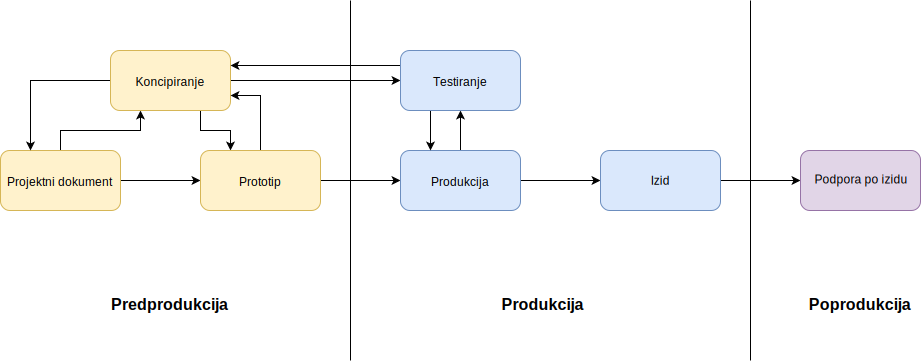
\includegraphics[width=15cm]{LifeCycle}
	\caption{Koraki razvoja igre}
	\label{slika:lifeCycle}
	\vspace*{-2em}
\end{figure}
\begin{enumerate}
	\item \textbf{Projektni dokument}. Tukaj preide ideja iz glave na fizični medij. Proces je zelo odvisen od velikosti projekta in studia. Pri večjih projektih nastane dejanski dokument, v katerem se definira ideja, kake bodo mehanike igre, zgodba, liki, razporeditev sredstev, predviden čas izdelave, ipd. Dokument je velikokrat tudi opremljen z konceptnimi slikami, ki jih pripravijo umetniki. S tem dokumentom je potem najlaže komunicirat vizijo preostalim ljudem v ekipi. Pri manjših idejah in posameznikih je ta korak bolj direkten. Ustvarijo se kake skice in krajši opisi, ampak večinoma pa se ta korak preskoči in je večji poudarek na prototipu.
	\item \textbf{Prototip}. Je najpomembnejši korak v procesu razvoja igre. Sama definicija pomeni razvoj osnovnega produkta, ki je ustvarjen z namenom testiranja koncepta \cite{blackwell2015prototype}. Glavni namen je preizkusit, ali je glavna ideja igre dovolj dobra, da iz nje nastane končni produkt. Prototipiranje je zelo povezano z samim koncipiranjem in projektnim dokumentom. Tukaj se identificirajo pomanjkljivosti, ki jih je potrebno razčistiti in mogoče znova koncipirati, ter prednosti, ki jih je potrebno poudariti v končnem produktu. Dober prototip je odličen mejnik v razvoju, ki se uporablja kot izhodiščna točka za začetek pravega projekta. Obenem služi kot prikaz koncepta možnim investitorjem, ki bi hoteli vložiti v projekt. 
	\item \textbf{Produkcija}. Je glavni del razvoja projekta. Sodelujejo vsi člani ekipe opisani v poglavju \ref{sec:opis_problema}. Konstantna komunikacija med razvijalci, preizkuševalci in oblikovalci pelje projekt skozi faze razvoja programske opreme: \textit{pre-alpha, alpha, beta, release candidate, live release (gold)}. Odvisno od projekta, se lahko studio odloči, da izdajo produkt končnim uporabnikom še v fazi razvoja. Tako postanejo uporabniki del preizkuševalcev, ki pomagajo pri razvoju projekta.
	\item \textbf{Izid}. Pomeni konec glavnega procesa razvoja. Igra se zapakira in distribuira do končnih uporabnik preko posrednikov. Ker mine kar nekaj časa od verzije, ki jo razvijalci dajo distribuiran na fizičnih medijih, do dejanskega izida, je danes ustaljena praksa prenos popravkov preko spleta na dan izida. Nekoč se je tukaj razvoj igre zaključil, razvijalci pa so prehajali na naslednji projekt. Dandanes pa izid pomeni le še en mejnik v samem življenjskem ciklu igre.
	\item \textbf{Podpora po izidu} . Tako imenovan \textit{post production} v angleščini postaja danes vedno večji faktor. Razvoj igre je veliki finančni podvig, ki največ sredstev terja do izida igre. Zato se veliki studii raje posvetijo izdani igri z nadaljnjo podporo. Začel se je uporabljati termin igre kot storitev (angl. \textit{games as a service}). Studii podpirajo igro še vrsto let z novimi vsebinami, popravki ter včasih korenitimi spremembami s ciljem maksimirati dobiček. Konstantna komunikacija z ciljno publiko je pomembna, saj tako identificirajo, kaj si igralci želijo novega v igri.
\end{enumerate}
Zgornji koraki so vidni v sliki \ref{slika:lifeCycle}. Kot vidno je proces razvoja, testiranja in koncipiranja zelo povezan, saj se igra konstantno izboljšuje.

\section{Marketing in viri občinstva}
Uspešna izdaja računalniške igre je zelo odvisna od marketinga pred izidom. Brez marketinga je zelo težko, da bo kdo našo igro opazil, kaj šele kupil. Samo na igralni platformi Steam letno izide več kot 6000 iger \cite{james6000Games}. V tej množici je pomembno, da naša igra izstopa in prav tukaj je zelo pomemben marketing že v zgodnjih fazah razvoja. Dober začetek marketinga je, ko lahko pokažemo glavne koncepte igre. Velikokrat so to slike ali videi igre v gibanju, ki pritegnejo končnega uporabnika \cite{robertMarketing}.

Obstaja veliko različnih načinov marketinga. Spodaj našteti so dandanes že skoraj obvezni, če hočemo uspeti na trgu \cite{robertMarketing}:
\begin{itemize}
	\item \textbf{Spletna stran.} Vsaka igra potrebuje svojo spletno stran. Brez le-te bo težko končna publika našla dodatne informacije o igri. Pomembno je, da stran vestno posodabljamo z opisom koncepta igre, slikami, videi, ipd. Ena možnost za hitro postavitev strani je \textit{presskit()} \footnote{http://dopresskit.com/}, prosto dostopen paket za enostavno stran za računalniško igro.
	\item \textbf{Blog.} Dober vir marketinga in občinstva je blog, kjer opisujemo potek razvoja igre. Veliko igralcev zanima, kako poteka razvoj in v katerem stanju se igra trenutno nahaja. Je tudi dober vir povezovanja z drugimi razvijalci, ki bi jih mogoče zanimalo sodelovanje na projektu. Paziti moramo le, da ne pretiravamo z objavami, saj ni vsak napredek v razvoju vreden omembe.
	\item \textbf{Socialni mediji.} Dandanes skoraj največja možnost pridobitve ciljnega občinstva so socialni mediji. Dobra stran igre na Facebook-u in kratke objave zanimive na Twitter-ju doprinesejo veliko. Socialna omrežja ponujajo tudi svoj plačljiv marketing s katerim lahko ciljamo specifično publiko, ki bi se zanimala za našo igro.
	\item \textbf{Konference.} Vsako leto poteka več konferenc, kjer se razvijalci predstavijo s svojimi igrami. Na konferenci se obrne veliko igralcev in različnih medijev, ki zelo pripomorejo k marketingu igre. Tri izmed večjih takih konferenc so Pax\footnote{http://www.paxsite.com/}, IndieCade\footnote{http://www.indiecade.com/} in Indie Mega Booth\footnote{http://indiemegabooth.com/}. V Sloveniji je največja konferenca SGC\footnote{http://sgc.si/}.
	\item \textbf{Množično financiranje (angl. crowdfunding).} Danes vedno bolj popularen način zbiranja sredstev in občinstva za razvoj igre. Preko strani kot je Kickstarter predstavimo svojo vizijo in načrt razvoja, ter tako poskusimo doseči igralce, ki bi jih zanimala naša igra. Ti pa lahko nato financirajo razvoj.
	\item \textbf{Napovednik (angl. trailer).} Ko se igra začne bližati zaključnim fazam razvoja je dobro izdelati napovednik, ki se bo potem uporabil na platformah, kjer bomo igro izdali. V napovedniku je pomembno, da prikažemo glavni koncept igre in da smo iskreni. Zavajajoči napovedniki lahko ustvarijo večjo začetno zanimanje vendar po izidu hitro pritegne slabo kritiko.
\end{itemize}

\section{Možnosti izdaje igre}
Opisali smo nekaj možnosti, ki so nam na voljo za izdajo igre kot individualnemu razvijalcu. Večina teh možnosti predvideva, da nimamo svojega distributerja in so zato najbolj primerne za manjše projekte:
\begin{itemize}
	\item \textbf{Steam.} Največja platforma za digitalno distribucijo računalniških iger. Omogoča izgradnje svoje strani za našo igro z vsemi potrebnimi informacijami. Sama platforma poskrbi za distribucijo, namestitev, posodobitve, varnostno kopijo shranjenih iger, glasovno komunikacijo v igri ipd. Na voljo je na vseh večjih operacijskih sistemih kot so Windows, OSX in Linux. Če se odločimo, da bomo našo igro izdali na Steam platformi, nam Steam ponudi implementacijo njihovega SDK, ki nudi proti-piratsko rešitev, mikro transakcije, oblačne storitve, dosežke ipd. Cena za izdajo igre je 100 evrov, provizija za vsako prodano kopijo igre pa je 30\% \cite{steam}.
	\item \textbf{Itch.io.} Zelo popularna rešitev za individualne razvijalce, saj ne stane nič, da svojo igro dodamo na njihovo platformo. Podobno kot Steam ponujajo izgradnjo svoje strani za igro ter aplikacijo, ki skrbi za namestitve in posodobitve. Platforma ne ponuja svoj SDK, ki bi nudil dodatne funkcionalnosti. Možno je nastaviti minimalno ceno igro, kupci pa lahko po želji plačajo več. Provizija je 10\% od vsakega nakupa, po želji pa lahko povečamo ta delež \cite{itchiofaq}.
	\item \textbf{Humble Bundle.} Ponuja tri vrste prodaje skozi njihovo platformo. Prva možnost je izgradnja zastonj strani, kjer ponujamo svojo igro. Oni poskrbijo za transakcije in si vzamejo 5\% provizije. Ta stran je neodvisna od njihove trgovine. Druga možnost je samostojen majhen gradnik, ki ga potem lahko dodamo na svojo spletno stran. Podobno kot pri njihovi neodvisni strani si vzamejo 5\% provizije. Zadnja možnost pa je prodajanje na njihovi spletni trgovini. Tukaj lahko dobimo njihovo izpostavitev naše igre, imamo znižanja ipd. So samo spletna trgovina, ne ponujajo aplikacije za prenašanje in posodabljanje iger. Provizija za prodajo v njihovi trgovini je 25\%, ne stane pa nič, da svojo igro objavimo \cite{humblebundle}.
	\item \textbf{GameJolt.} Podobno kot itch.io je zelo popularna platforma za neodvisne razvijalce. Nudijo svojo aplikacijo za prenose in posodobitve. Objava igre v njihovo trgovino ne stane nič, provizija pa je 10\% ali manj saj ponujajo možnost znižanja provizije. Promovirajo skupnost neodvisnih razvijalcev, zato vse dobičke dobimo na njihov račun, ki jih lahko nato porabimo za nakup iger drugih razvijalcev, brez dodatne provizije. Seveda je možno denar si vedno izplačati \cite{gamejolt}.
	\item \textbf{Apple store in Google Play.} Če je naša igra namenjena za mobilne naprave, potem moramo obvezno uporabiti ti dve trgovini. Obe nudita izgradnjo svoje strani za igro na trgovini, prenose, posodobitve in dodatne transakcije. Kot mobilna platforma ponujata tudi dodatni SDK, s katerimi lahko v našo igro vgradimo lestvice, nagrade, oblačne storitve ipd. Provizija je 30\% od nakupa, je pa potrebno tudi plačati za objavo aplikacije v trgovini. Pri Google Play je to enkratna cena 25 evrov, nakar lahko izdajamo koliko hočemo aplikacij \cite{googleplay}. Pri Apple store je cena 99 evrov na leto \cite{applestore}.
\end{itemize} 

\chapter{Orodja za izdelavo iger}
\thispagestyle{fancy}
\section{Načrtovanje in vodenje razvoja}
Dobra organizacija veliko prispeva za tekoč razvoj računalniške igre. Obstaja veliko različnih orodij, nekatere so usmerjene za organizacijo ljudi in opravil, druge za organizacijo projekta in kode. Tudi, če samostojno razvijamo igro nam ta orodja veliko pomagajo, zato smo poiskali dobre rešitve in jih tudi opisali.

\subsection{Organizacija ljudi in opravil}
Delo je priporočljivo razdeliti na manjša opravila, ki jih lahko opišemo, razdelimo med skupino in vodimo njihov napredek. Dve izmed boljših orodij za to sta Trello in HackNPlan. Obe pa uporabljata principe kanban razvojnega sistema.

\begin{figure}[h]
	\centering
	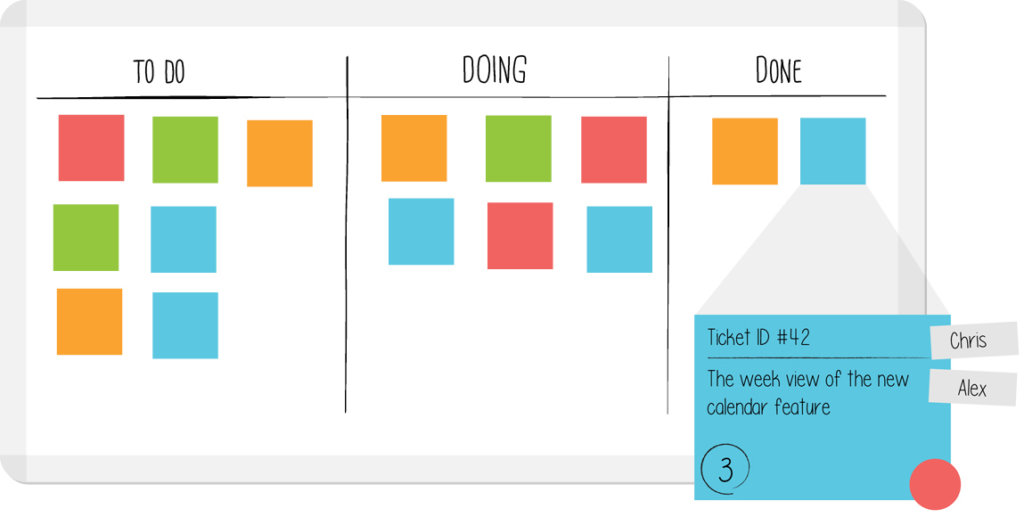
\includegraphics[width=10cm]{kanban_guide_print_KPO_bleed_board2}
	\caption{Kanban tabla. Vir \cite{kanbanBoard}}.
	\label{slika:kanbanBoard}
	\vspace*{-2em}
\end{figure}

Kanban sistem je način organizacije dela, katerega cilj je izboljšati ravnovesje med povpraševanjem in kapaciteto človeškega dela, ki je na voljo. Delo je razdeljeno na manjše kose in vizualizirano na kanban tabli kot primer na sliki \ref{slika:kanbanBoard}. Opravila so večinoma vizualizirana na listkih, ki hranijo potrebne podatke kot so naslov, opis, ocenjen čas potrebnega dela, trenutni upravitelji ipd. Ta opravila so uvrščena na pripadajoč del table, odvisno v kakem stanju je opravilo (npr. čaka na dela, v razvoju, v testiranju, potrebno ocene, končano, ipd.). Glavni cilj take organizacije je vizualizirati in kategorizirati opravila, ki jih nato razvijalci prevzamejo in opravijo \cite{kanbanBoard}.

Trello je produkt pod okriljem podjetja Atlassian, ki med drugim nudijo storitve kot so Jira in BitBucket. Ponuja nam izgradnjo tabel, na katera dodajamo opravila v obliki kartic z vsemi potrebnimi informacijami. Razvijalce lahko razvrstimo v skupine in tabele, nakar se lahko dodelijo na opravilo. Primer demo table je viden na sliki \ref{slika:trelloDemo}. Storitev je na voljo preko spletne strani, ponujajo pa tudi mobilno aplikacijo. Vsa funkcionalnost je na voljo zastonj, z možnostjo nadgradnje za 9.99 dolarjev za vsakega člana na mesec. Nadgradnja nam omogoči nalaganje večjih datotek, dodatne varnostne funkcionalnosti, prvo ročno pomoč od podjetja ter več integracij za vsako tablo. Integracije so na voljo z njihovimi in drugimi produkti za lažjo organizacijo. Zastonjska verzija je za individualni razvoj več kot dovolj, saj so nadgradnje namenjene za večje projekte in skupine.

\begin{figure}[h]
	\centering
	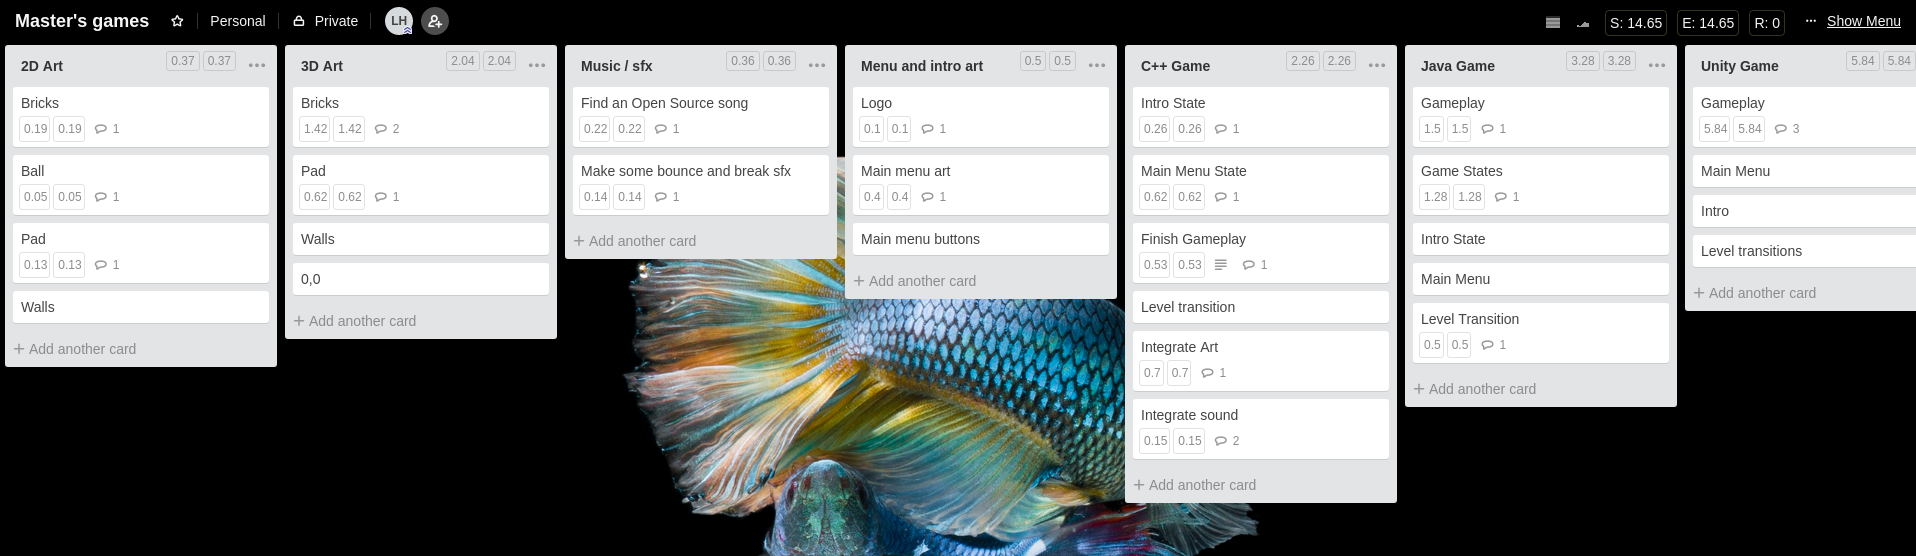
\includegraphics[width=10cm]{trelloBoardDemo}
	\caption{Primer Trello table.}.
	\label{slika:trelloDemo}
	\vspace*{-2em}
\end{figure}

HackNPlan je v osnovi podoben kot Trello, vendar je zgrajen specifično za razvoj računalniških iger. Poleg kanban table in organizacije ljudi ponuja še preglede statistik, vodenje sprintov ter funkcionalnost za skupno koncipiranje in dokumentiranje idej. Primer table vidimo na sliki \ref{slika:hacknplanDemo}. Vso našteto funkcionalnost dobimo v zastonjski verziji ponujajo pa tudi nadgradnjo za dodatne storitve. Cena nadgradnje je 4 evre na mesec in glavna dodatna funkcionalnost so integracije z drugimi storitvami kot so GitHub, Slack, ipd. Zastonjskih integracij ni, zato je na tem področju slabši produkt kot Trello, vendar pa specifične funkcionalnost za namen razvoja iger veliko pripomorejo.

\begin{figure}[h]
	\centering
	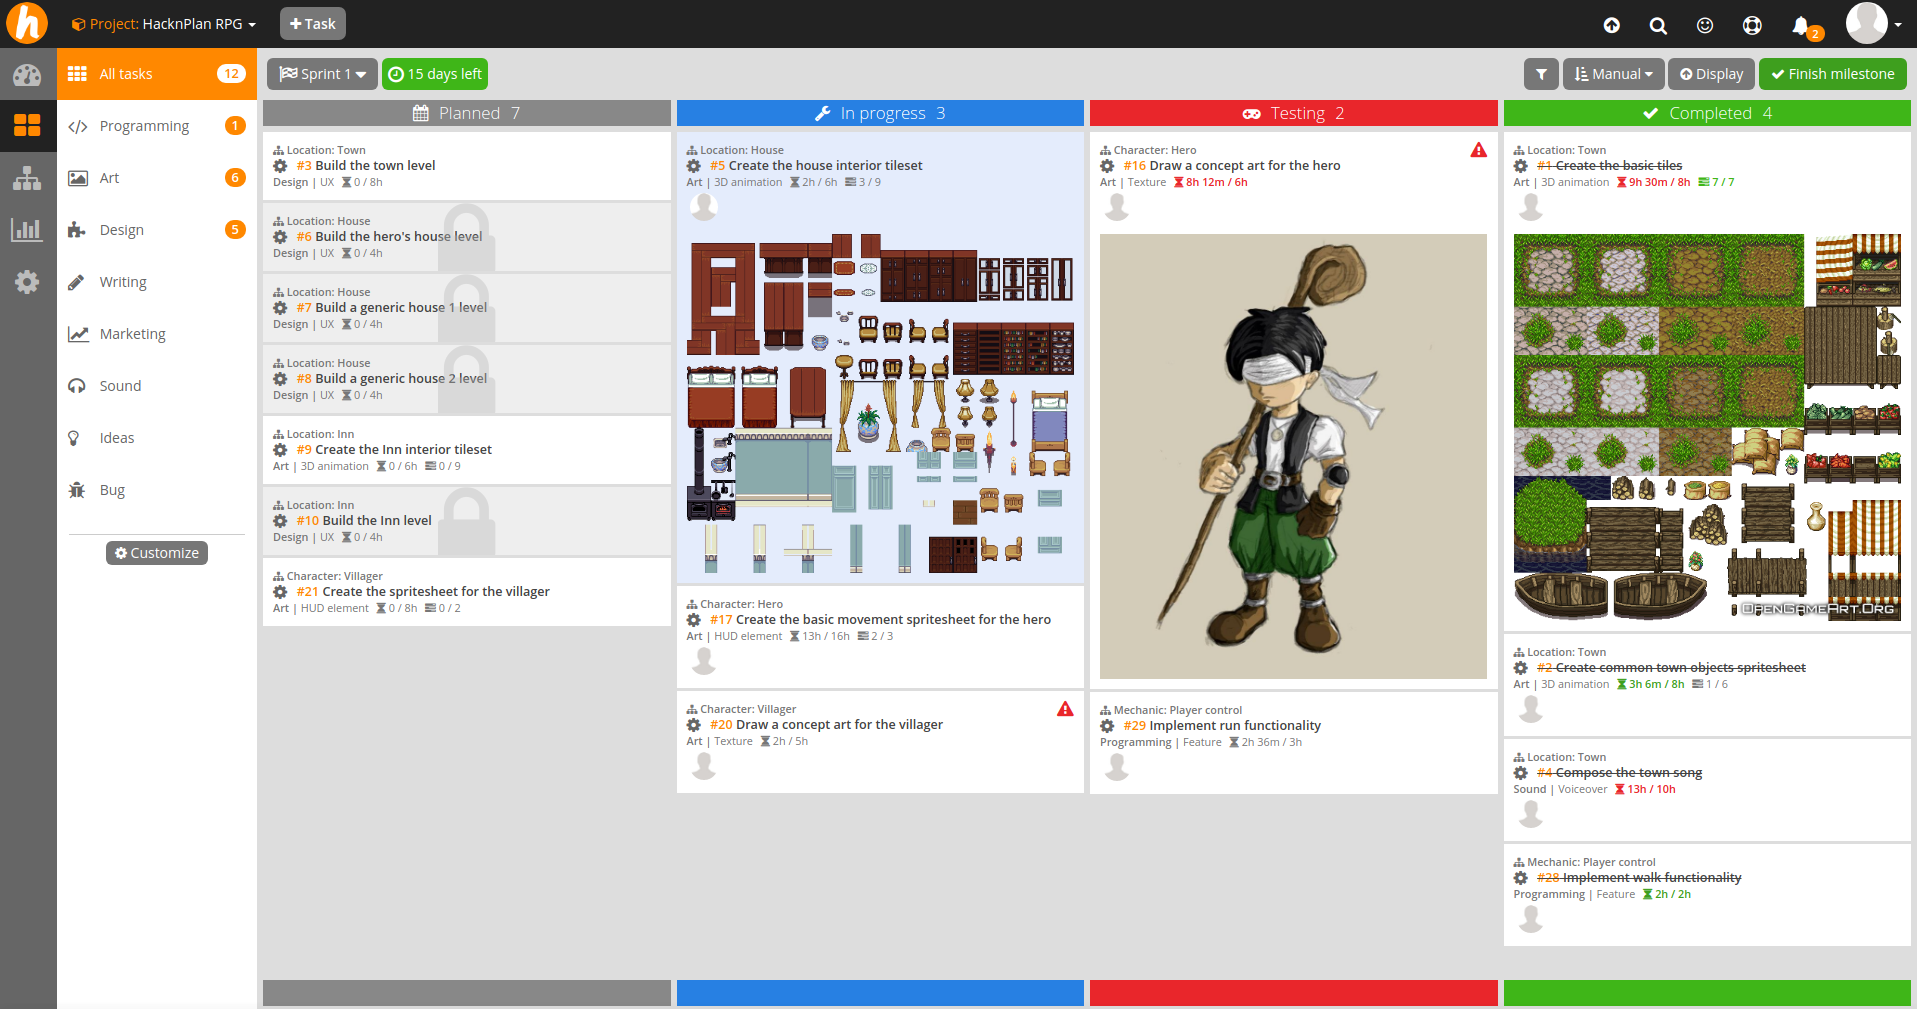
\includegraphics[width=13cm]{hacknplanDemo}
	\caption{Primer HackNPlan table.}.
	\label{slika:hacknplanDemo}
	\vspace*{-2em}
\end{figure}

\subsection{Organizacija projekta in kode}
Enako pomembno kot organizacija opravil je organizacija samega projekta med razvojem. Za te potrebe obstaja več rešitev verzioniranja projektov kot so SVN, Mercurial, GIT, Perforce, itd. Te programske rešitve ponujajo način hranjenja trenutnega stanja projekte kode na centralnem mestu, obenem pa sledijo vsem spremembam vsake datoteke. Mogoče je tudi hraniti več različnih aktualnih verzij iste datoteke v različnih vejah, in jih nato združiti v končno obliko. Vsak razvijalec ima lokalno svojo kopijo projekta in svoje spremembe pošilja v centralni repozitorij. Tako v ozadju nastaja drevesna struktura sprememb projekta skozi čas. Primer takega grafa vidimo na sliki \ref{slika:gitGraph}. Vsaka sprememba je komentirana s strani razvijalca in tako je možno hitro poiskati in preiti na starejšo verzijo v primeru težav \cite{versionControl}.
	
\begin{figure}[h]
	\centering
	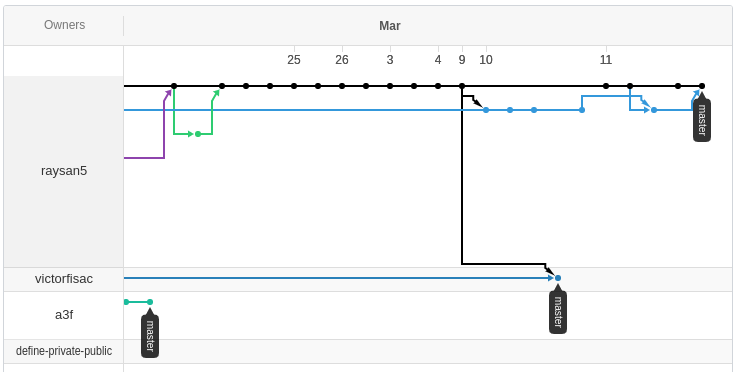
\includegraphics[width=13cm]{gitGraph}
	\caption{Primer grafa sprememb Raylib projekta na GitHub-u.}.
	\label{slika:gitGraph}
	\vspace*{-2em}
\end{figure}

V industriji razvoja računalniških iger je najbolj uporabljen sistem verzioniranja Perforce, saj deluje najboljše za večje projekte in kot komercialna plačljiva programska rešitve ponuja zelo močna orodja za delo z binarnimi datoteka (umetniški in zvočni gradniki so velikokrat v binarnem formatu in obenem največje datoteke v projektu). Za večje projekte je Perforce plačljiv, ponujajo pa zastonjsko različico za projekte do 5 ljudi.

Najbolj preprost za uporabo in najbolj razširjen pri razvoju programske opreme pa je sistem Git. Popularnost je v veliki meri povezana s storitvijo GitHub, ki ponuja oblačno hranjenje repozitorija z našim projektom, obenem pa nudi funkcionalnost za lažje skupno delo na projektu. Alternativa GitHub-u je BitBucket, obe rešitvi pa smo analizirali za potrebe razvoja igre.

GitHub je spletna platforma zgrajena na bazi sistema verzioniranja Git. Glavna storitev je gostovanje našega repozitorja v oblaku, vendar imajo še obilo drugih storitev zaradi česar so zelo priljubljeni za veliko projektov. Omogočajo upravljanje z ljudmi in skupina, kdo ima dostop do kode, kdo dela na čem ipd. Pregled sprememb je preprost za uporabo in omogoča komentiranje nad kodo. Za vsak projekt nudijo tudi sistem sledenju napak (npr. kot Bugzilla), kjer lahko vsi, ki uporabljajo programsko opremo javijo napake in komunicirajo z razvijalci. Zelo popularna funkcionalnost so tudi zahteve za spremembe (angleško \textit{pull request}), kjer lahko nekdo izdela in predlaga spremembe za projekt, nato pa se razvijalci odločijo, ali bodo te spremembe integrirali v glavno vejo projekta. Za odprtokodne in javne projekte je vsa za funkcionalnost zelo dobrodošla, saj nudi lažje upravljanje z projektom. Zastonjska verzija Github-a ponuja vso našteto funkcionalnost, omejitev je le v tem, da morajo vsi naši projekti biti javni. Če hočemo imeti zasebni projekt na Github, potem je potrebno plačat 7 evrov mesečno \cite{github}.

Alternativa Github-u je storitev BitBucket. Ponuja enako funkcionalnost vendar v zastonjski storitvi dovolijo zasebne repozitorije. Omejitev zastonjskega paketa je maksimalno 5 razvijalcev na projektu. Če hočemo povečati število razvijalcev je cena 2 evra na razvijalca na mesec. Za projekte z manjšo skupino je torej BitBucket boljša rešitev za privatni repozitorij. Če pa hočemo, da je naš projekt na voljo vsem, je pa boljša alternativa GitHub \cite{bitBucket}.

\section{Orodja za izdelavo grafičnih gradnikov}
Grafični gradniki so pri razvoju računalniške igre uporabljeni od samega koncipiranja do končnega izida igre. Mi smo se osredotočili na gradnike, ki se uporabijo v sami računalniški igri. Ti gradniki so odvisno od tipa igra 2D slike ali 3D modeli. Na trgu obstaja veliko rešitev za izdelavo teh gradnikov, mi pa smo analizirali zastonjsko programsko opremo, ki ima več kot dovolj funkcionalnosti za izdelavo potrebnih gradnikov za individualne projekte.

\subsection{2D grafični gradniki}
Individualni projekti večinoma uporabljajo dva stila 2D grafičnih gradnikov. Angleško imenovana \textit{pixel art} in \textit{vector art} (slovensko vektorska umetnost). Končni rezultat je kljub imen vedno rastrska slika, razlika je kako so gradniki ustvarjeni in kaj je v stilu pomembno. Pixel art izhaja iz navdiha iz starih igralnih sistemov, kjer so bile omejitve v smislu resolucije gradnikov in razpoložljivosti barv. Pomembno je izkoristiti vsak piksel, ki je na voljo. Vektorski gradniki pa v nasprotju ciljajo na gradnike višje resolucije. Poskušajo uporabiti preproste oblike in združevanje le-teh za pridobitev končnih slik. Razliko v stilih vidimo na sliki \ref{slika:pixelVsVector}.

\begin{figure}[h]
	\centering
	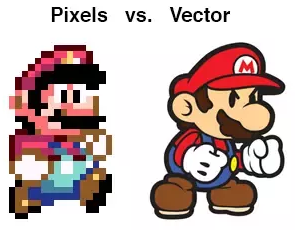
\includegraphics[width=6cm]{pixelVsVector}
	\caption{Razlika v stilih 2d grafičnih gradnikov. Vir \cite{pixelVsVector}}
	\label{slika:pixelVsVector}
\end{figure}

Program, ki ga priporočamo za izdelavo 2D pixel art gradnikov je Aseprite\footnote{https://www.aseprite.org/}. Vsa potrebna funkcionalnost za delo z slikami iz profesionalnih programov je na voljo, vendar so vse prilagojene za delo s slikami nižjih resolucij. Zelo močna so tudi orodja za delo z animacijami, plastmi, ipd. Za namen razvoja računalniških iger nam ponuja tudi posebne izvoze v teksturne atlase in nize slik za animacijo. Program je na voljo za 15 evrov, vendar je vsa izvorna koda javna. Uradno da si lahko sami zgradimo program in ga uporabljamo v komercialne namene. Prednost plačljive različice so samodejne posodobitve, ni potrebno prevajati izvorne kode ter seveda podpora nadaljnjega razvoja.

Za razvoj vektorske grafike pa predlagamo program Inkscape. Po funkcionalnost je podoben Adobe Illustrator-ju, le da je na voljo kot zastonjska odprtokodna rešitev. Manjkajo napredne funkcionalnosti koz je zvijanje združenih objektov za potrebe animacije, vendar na trgu ni boljše zastonjske alternative. V Inkscape delamo z vsemi liki kot z objekti, in nad njimi lahko izvajamo booleanove transformacije (presek, unija, odštevanje, ipd.) ter tako ustvarimo željene like. Ker delamo z objekti je naš končni izdelek neodvisen on resolucije in ga lahko izvozimo v željeni velikosti za našo igro. 

\subsection{3D grafični gradniki}
Izdelava 3D modelov je bolj zahtevna od 2D gradnikov saj je potrebnih več korakov (modeliranje, teksture, animiranje). V industriji se uporabljajo različni programski paketi kot so Maya, Houdini, ZBrush in Blender. Od teh je Blender edini zastonjski in odprtokodni program. V zadnjih letih je vedno bolj uporabljen v industriji, saj se s svojo funkcionalnostjo lahko kosa z drugimi plačljivimi programi in jih na določenih mestih celo preseže. 

\section{Orodja za izdelavo zvočnih gradnikov in glasbe}

\section{Računalniške knjižnice, ogrodja in pogoni}

\chapter{Razvoj računalniške iger}
\thispagestyle{fancy}

\chapter{Sklep}
\thispagestyle{fancy}

\cleardoublepage
\bibliographystyle{plain}
\bibliography{thesis}
\addcontentsline{toc}{chapter}{Literatura}
\thispagestyle{fancy}

\end{document}













